%
% teil1.tex -- Beispiel-File für das Paper
%
% (c) 2020 Prof Dr Andreas Müller, Hochschule Rapperswil
%
\section{Beschrieb des Zuordnungsproblems
\label{munkres:section:teil1}}
\rhead{Problemstellung}

Das spezielle an einem Zuordnungsproblem ist, dass es an jedem Ort nur eine Einheit angeboten bzw. nachgefragt wird. Es werden hier nicht Mengen möglichst kostenminimal von einem zum anderen
Ort transportiert, sondern es geht um die kostenminimale Zuordnung von z.B. Personen, oder Bau-Materialien auf bestimmte Orte, Stellen oder Aufgaben.
Um dieses Problem in einer einfachen, händischen Art und Weise zu lösen wurde der Munkres-Algorithmus, auch die Ungarische Methode genannt, entwickelt. Diese Methode ist ein weiteres Hauptthema dieses Kapitels.

\subsection{Zuordnungsproblem an einem konkreten Beispiel
\label{munkres:subsection:bonorum}}

\subsection{Zuordnungsproblem abstrakt
\label{munkres:subsection:bonorum}}

Es sind alle Angebots- und Bedarfsmengen gleich 1 
\begin{equation}
a_{i}=b_{j}=1
\end{equation}

\subsection{alternative Darstellungen des Zuordnungsproblems
\label{munkres:subsection:bonorum}}
\begin{equation}
Netzwerk
\end{equation}
\begin{equation}
Matrix
\end{equation}
\begin{equation}
Bitpartiter Graph
\end{equation}
Ein bipartiter Graph ist ein mathematisches Modell für Beziehungen
zwischen den Elementen zweier Mengen.
Es eignet sich sehr gut zur Untersuchung von Zuordnungsproblemen» 
\begin{figure}
\centering
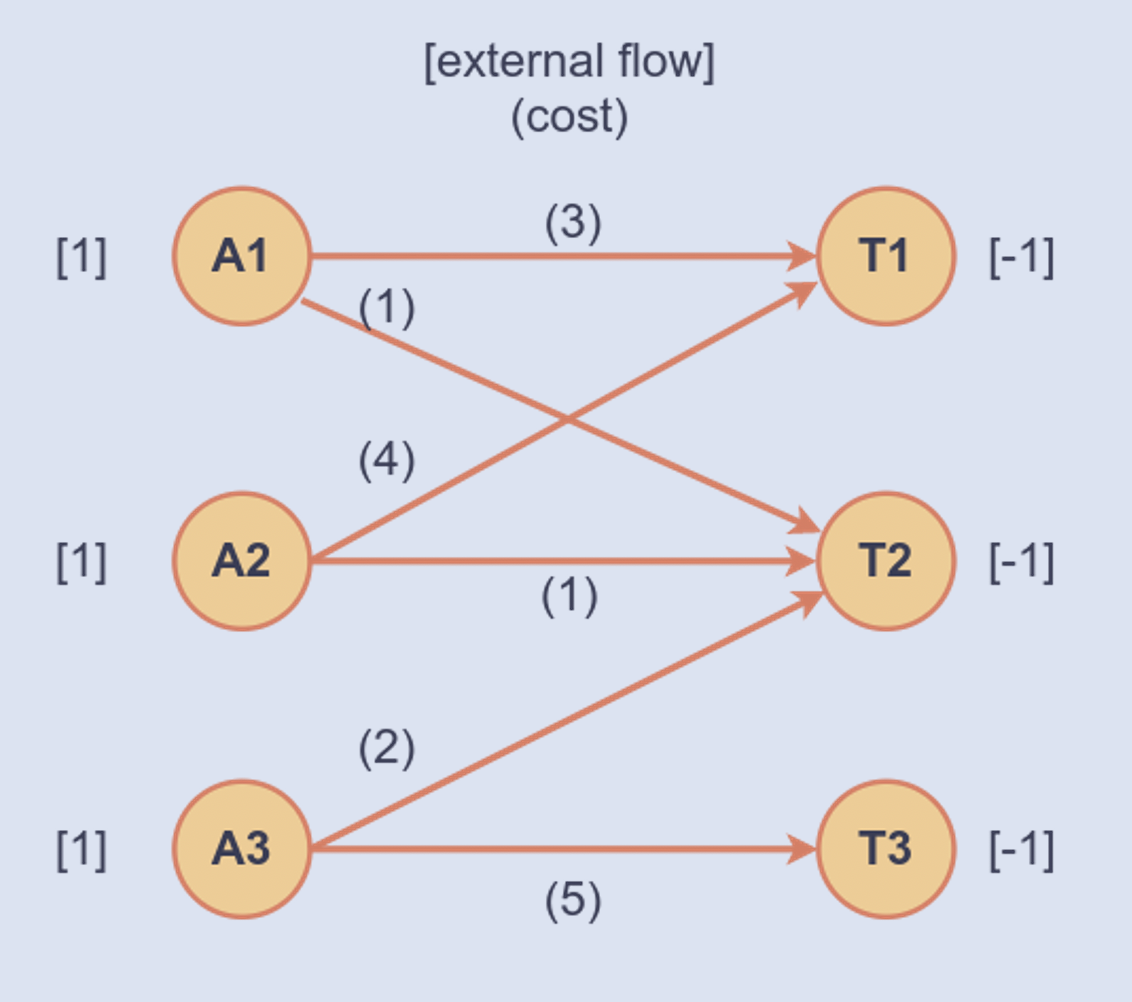
\includegraphics[width=5cm]{papers/munkres/figures/Netzwerkdarstellung}
\caption{Typische Netzwerkdarstellung eines Zuordnungsproblems.}
\label{munkres:Vr2}
\end{figure}

\begin{figure}
\centering
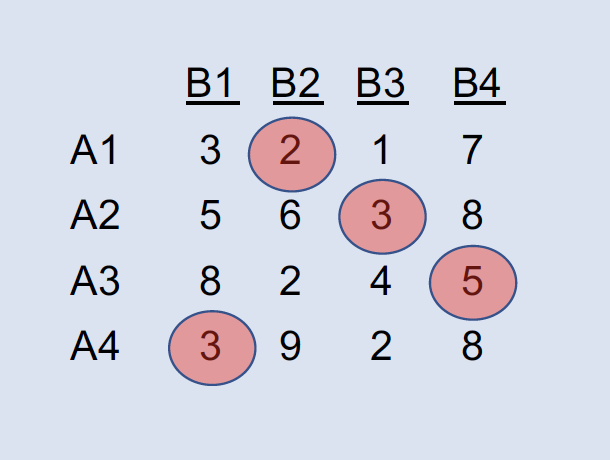
\includegraphics[width=5cm]{papers/munkres/figures/Matrixdarstellung}
\caption{Typische 4x4 Matrixdarstellung eines Zuordnungsproblems.}
\label{munkres:Vr2}
\end{figure}

\begin{figure}
\centering
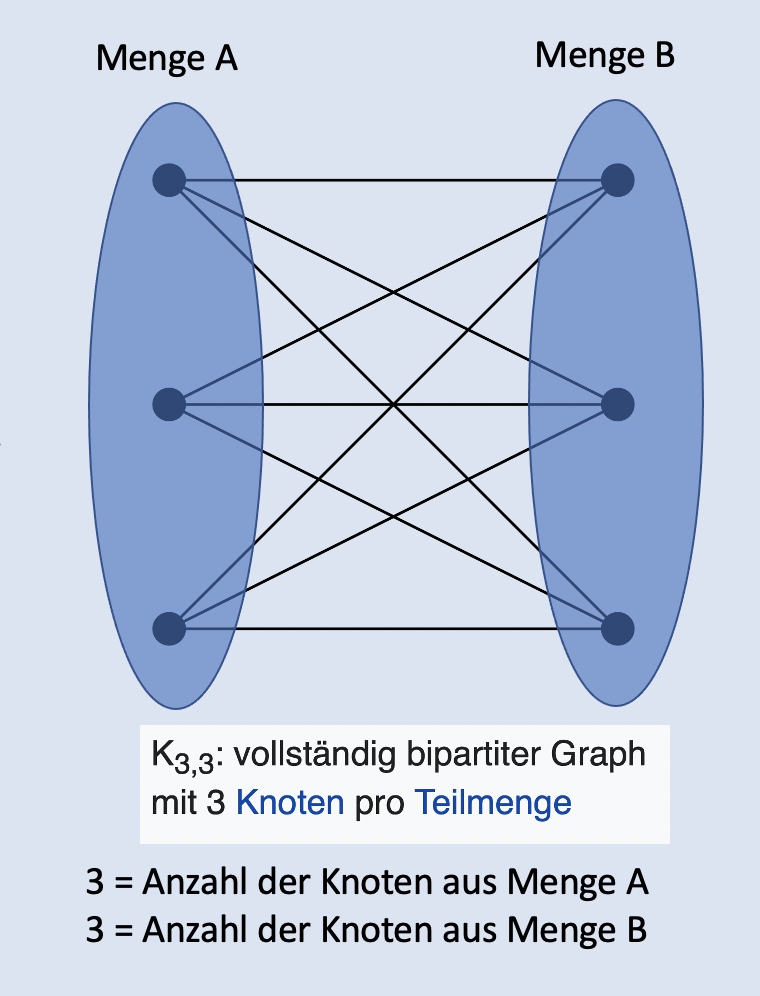
\includegraphics[width=5cm]{papers/munkres/figures/bipartiter_graph}
\caption{$K_{3,3}$ vollständig bipartiter Graph mit 3 Knoten pro Teilmenge.}
\label{munkres:Vr2}
\end{figure}
